\section{Auswertung}
\subsection{Kennlinie der Pumpe}
Damit die Pumpenkennlinie dargestellt werden kann, müssen die gemessenen Ströme für den Volumenstrom und den Druck erst in verwwendbare Einheiten umgewandelt werden. 
Hierzu werden Proportionalitätsfaktoren und Kalibrieungsoffsets benötigt. 
Die Offsets wurden gemessen und batragen $I_{off,Q}=4,05 mA$ und $I_{off,p}=5,868 mA$.
Die Proportionalitätsfaktoren wurden in der Versuchsanleitung gegeben und betragen $K_Q = 6,3 \frac{l}{min \cdot mA}$ und $K_p = 0,6 \frac{bar}{mA}$.
Die Volumenströme in $\frac{m^3}{h}$ lassen sich mittels \autoref{eq:230513_Volumenstrom} berechnen und die Drücke in bar mittels \autoref{eq:230513_Druck}.
\begin{equation}
  Q = (I_{mess}-I_{off,Q})\cdot K_Q \cdot \frac{60\frac{min}{h}}{1000\frac{l}{m^3}}
  \label{eq:230513_Volumenstrom}
\end{equation}

\begin{equation}
  p = (I_{mess}-I_{off,p})\cdot K_p
  \label{eq:230513_Druck}
\end{equation}

Des wieteren müssen die Drücke in Förderhöhen umgewandelt werden. Hierzu wird die gravitationknostante $g = 9,81 \frac{m}{s^2}$ und die Dichte des Wassers $\rho = 998 \frac{kg}{m^3}$ benötigt.
Dies erfolgt mit \autoref{eq:230513_Förderhöhe}, wobei der Druck in Pascal und nicht in bar angegeben werden muss.

\begin{equation}
  H = \frac{p}{\rho \cdot g}
  \label{eq:230513_Förderhöhe}
\end{equation}

Aus den im Anhang gegebenen Messtabelln ergibt sich die \autoref{fig:230513_Pumpenkennlinie}.
\begin{figure}[!ht]
  \centering
  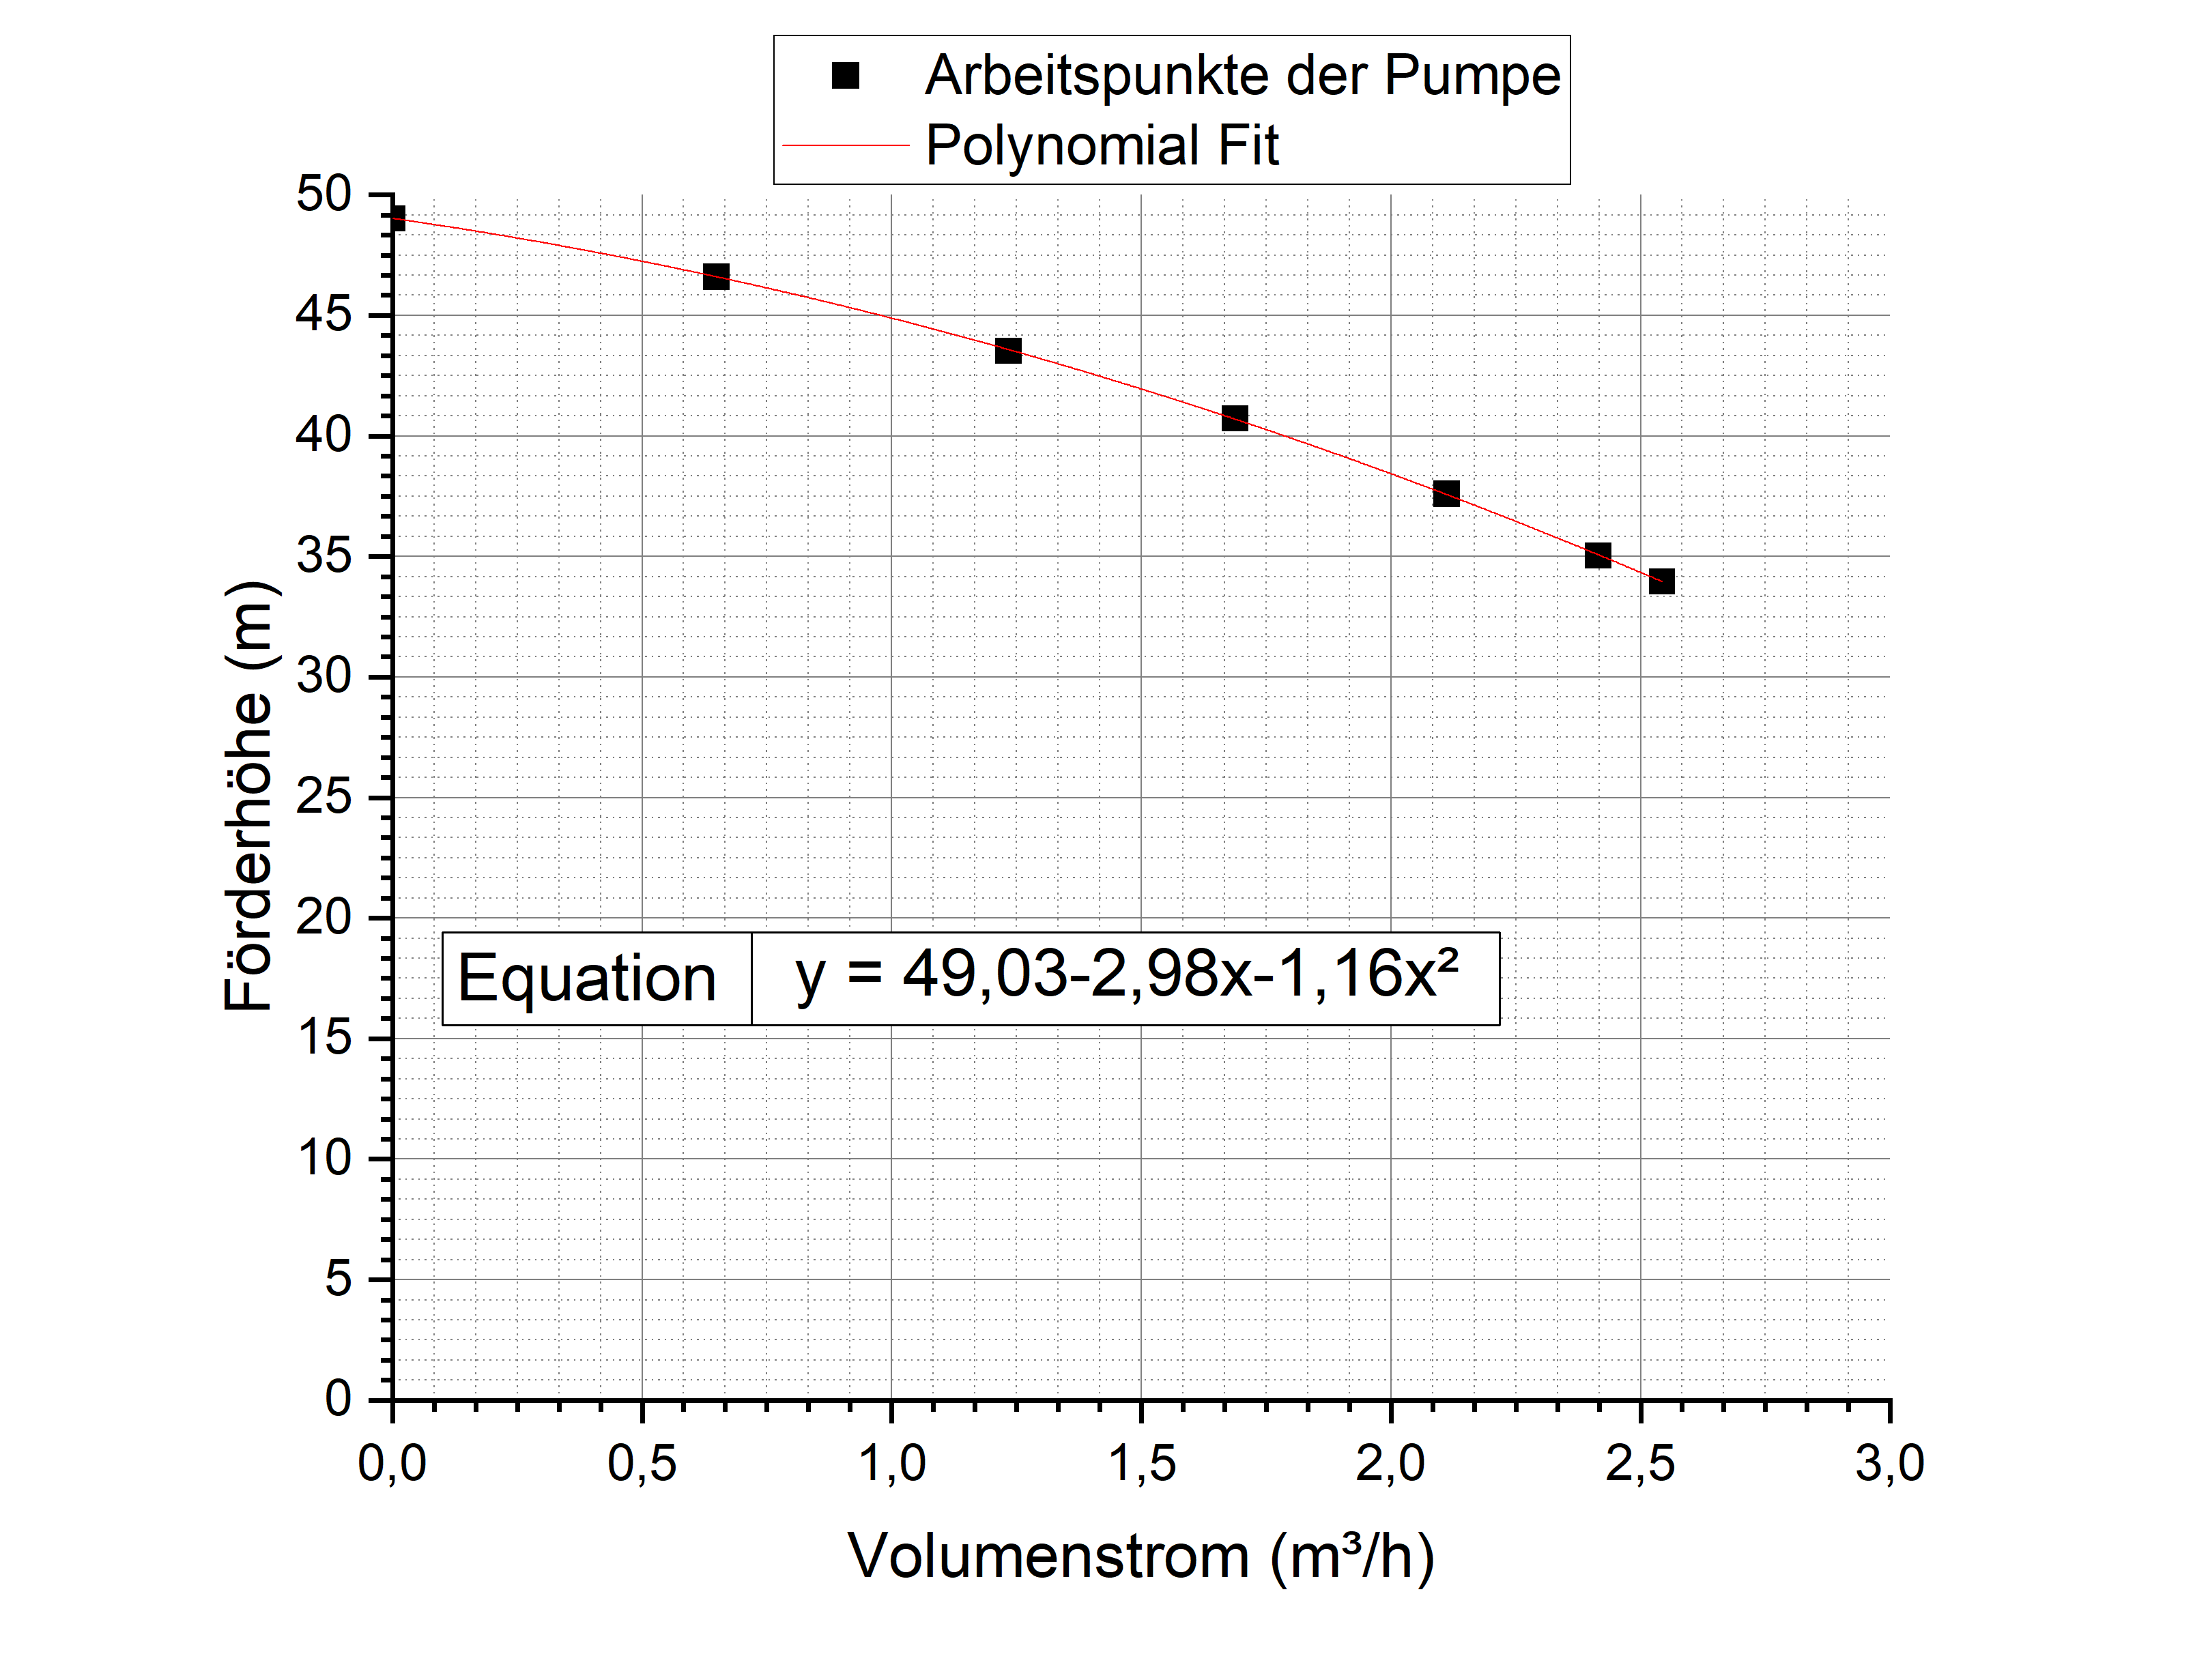
\includegraphics[width=0.8\textwidth]{Abbildungen/Pumpenkennlinie.png}
  \caption{Pumpenkennlinie bei gemessenen Arbeitspunkten}
  \label{fig:230513_Pumpenkennlinie}
\end{figure}

\subsection{Betriebspunkte der Pelton-Turbine}
\subsection{Verlustbeiwert der Düse}